\chapter{Description of Problem}
\label{sec:description}

Our problem was to design a snapshotting system for Ceph that asynchronously
replicates data to remote data centers. In this chapter, we discuss the details
of the problem and the constraints that were placed on our solution. 

\section{Ceph}

The architecture and requirements of Ceph place a lot of constraints on our
solution. Ceph is a distributed file system, meaning that data is stored in
many different nodes in a Ceph cluster. There
is no central node through which all read and write requests are sent. 
Instead, reads and write requests are sent directly to the nodes that contain
the relevant data. This means that there is no centralized log of all of the
reads/writes events that the Ceph cluster handles.

Ceph maintains very strong consistency guarantees on the data that's 
stored in its system. It is designed to replicate data on multiple nodes, such 
that one node's failure will not cause a permanent loss of data. This will 
maintain a user's data, even though it is common for nodes to fail in a large 
data center. Ceph will also hold a
confirmation of a write's success until it is certain that the data has been 
stored and properly replicated. When a client receives a confirmation of a write, they can be certain that the data has been received and replicated properly. These characteristics ensure that a user's 
data will be kept consistent.

Ceph also allows out-of-band communication for client applications. 
Out-of-band communication is communication that is related to the data in the 
Ceph cluster, but that Ceph cannot detect. This contrasts with in-band
communication, which the Ceph cluster can see and potentially account for. 

\begin{figure}[h]
  \centering
  \caption{~Two clients communicating with each other out-of-band.} 
  \label{fig:out-of-band}
  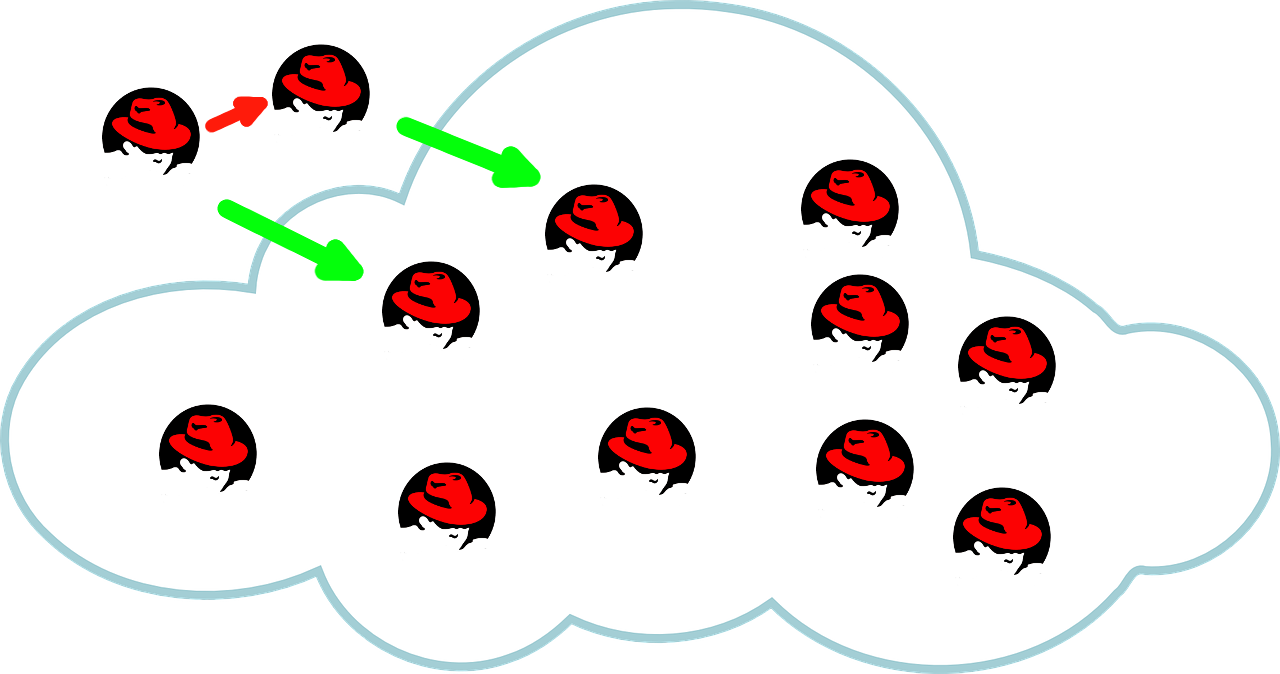
\includegraphics[width=0.8\textwidth]{outofbandwrite.png}
\end{figure}

For example, a pair of clients could be separately accessing a pair of data 
objects in the Ceph file system (see Figure~\ref{fig:out-of-band}). These clients could both be acting on behalf 
of the same application. Let's say the application is a text editor. The 
application may read from (or write to) a text file through the first client. 
As a result of this operation, the application then may decide to write to the 
second text file through the second client. Since these operations are handled 
by separate clients, Ceph cannot be certain of a causal relationship between 
the two events. 

In addition, Ceph is a very performant system. Currently, writes to a Ceph 
cluster take 4 to 20 milliseconds to perform~\citep{Sage}. Any solution that 
we provide must maintain Ceph's performance, which means that its read/write 
capabilities cannot be interrupted for extended periods of time.

Finally, Ceph allows a user to use any commodity hardware when constructing 
their cluster. This gives users more versatility, but adds extra constraints 
on our problem, since we cannot specify hardware that the user must purchase 
for a solution to work.

\section{Consistent Snapshots}

Our solution will require us to record the global state of the data in a Ceph 
cluster. A recording of that global state is called a ``snapshot". However, we 
require that a snapshot be consistent. A consistent snapshot is one that 
preserves the causal relationships of the read/write events that it captures.
This means that, if an event is captured, then all events that caused that 
event must be captured as well. 

For example, let's say event $A$ caused event $B$. Then a consistent snapshot 
is one where, if event $B$ is captured, then event $A$ is captured as well. If
event $B$ were captured, but event $A$ was not, then any backup based on that
snapshot could cause errors in applications that are using that inconsistent
data. See Figure~\ref{fig:consistency} for examples of consistent and 
inconsistent snapshots.

\begin{figure}[h]
  \centering
  \caption{~Event A caused event B. The dashed line in the center represents the time when the snapshot took place. The first three cases are examples of consistent snapshots. The last case is an inconsistent snapshot.} 
  \label{fig:consistency}
  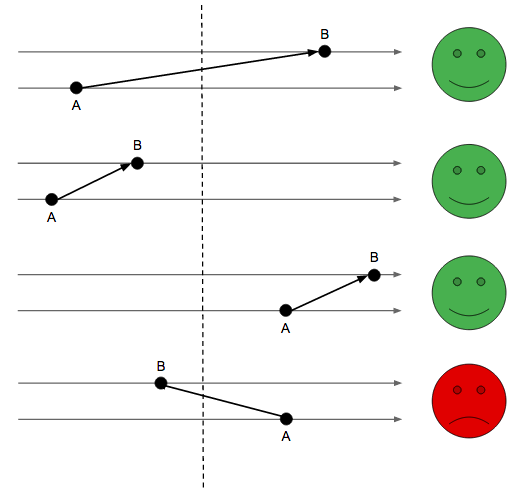
\includegraphics[width=0.75\textwidth]{consistency.png}
\end{figure}

\section{Snapshotting Complications}

The constraints described above make a snapshotting system not as intuitive as
it may initially seem.

Ceph's distributed architecture and lack of central log means that there is no
centralized place where we could obtain a total ordering of the events in our
cluster. A total ordering is an exact order of all events. Events
are logged on the individual nodes. This means that we will have to
use the partial data at each node to reconcile the ordering of the events, 
while still maintaining the consistency of the data in the system.

Logical clocks, like Lamport or vector clocks, are sometimes used to order 
events in distributed systems. They provide a partial ordering of the events in our system, which is
where events that have a causal relationship can be ordered. Ordinarily, these solutions could provide us a way to order events well enough to construct a consistent snapshot. However, they fail when
out-of-band communication is permitted. Since Ceph allows for out-of-band 
communication, Lamport and vector clocks will not work. For a more detailed explanation
of Lamport and vector clocks and why they do not solve our problem, see 
Chapter~\ref{sec:rel-work}.

We could also try to achieve ordering through timestamps. In theory,
this would be able to provide a total ordering of events. However, clocks are not perfect. Over time, clocks drift and become more desynchronized from each other. Ceph's distributed design means that each clock uses its own clock
when determining the timestamp of an event. Using the timestamps by themselves
will not allow us to get a total ordering of the events, since the clocks
would slowly become more and more desynchronized, until the clocks are no 
longer reliable ways to distinguish when events occured on different nodes. An 
event could receive a later timestamp than an event it caused, which could 
create an inconsistent snapshot of our system. 

Time synchronization protocols like the Network Time Protocol (NTP) could help
keep the clocks in our system from desynchronizing too greatly. However, no
time synchronization protocol we've been able to find can maintain 
clock synchronization well enough that would allow us to use timestamps alone
to order events consistently. However, we will see in Chapter~\ref{sec:approach} that other aspects of time synchronization protocols will prove useful
for our problem.

Another naive approach is to propagate a write freeze throughout the cluster. 
When a specific node determines that it is time to take a snapshot, it holds 
all incoming writes and messages its neighbors to do the same. This message 
is then sent through the center as each node does the same. In the end, when 
all nodes have frozen, the snapshot can be taken and the nodes begin to 
unfreeze. 

However, depending on the size of the cluster, it could take a long time for 
that freeze to propagate through the cluster. If a client wanted to write to  
the node that started the freeze, it could take tens of milliseconds to do so. 
This would noticeably degrade Ceph's performance, which is not acceptable. 
However, we will see in Chapter~\ref{sec:approach} that we can modify this 
approach to remove the performance degradation.

Finally, Google has implemented a library called TrueTime to provide ranges of 
what real time could be in their Spanner database. While this solution may seem like
it could work, it actually requires specific hardware, namely atomic and GPS
clocks, to function properly. Since Ceph can be running on any commodity hardware, we do
not want our solution to require specific hardware (though, as we'll see in 
Chapter~\ref{sec:impl}, specialized hardware can improve the performance of
our solution). Therefore, we cannot use TrueTime as a solution to this 
problem. For a more detailed explanation of TrueTime and why it does not solve 
our problem, see Chapter~\ref{sec:rel-work}.

% distributed architecture and no central log
% clock drift and timestamps
% logical clocks and out-of-band
% commodity hardware and true time













